In table \ref{effects1} and table \ref{effects2}, you can see the main effects and the interaction effects. As one can see, the effect of $B$ is a lot larger than the other effects. 

\begin{table}[H] \centering 
  \caption{Effects} 
  \label{effects1} 
\begin{tabular}{@{\extracolsep{5pt}} cccccccc} 
\\[-1.8ex]\hline 
\hline \\[-1.8ex] 
(Intercept) & A1 & B1 & C1 & D1 & A1:B1 & A1:C1 & A1:D1\\ 
$282.125$ & $$-$1.125$ & $$-$99.875$ & $12.875$ & $4.375$ & $$-$3.125$ & $2.625$ & $$-$3.875$\\ 
\hline \\[-1.8ex] 
\end{tabular} 
\end{table}

\begin{table}[H] \centering 
  \caption{Effects} 
  \label{effects2} 
\begin{tabular}{@{\extracolsep{5pt}} cccccccc} 
\\[-1.8ex]\hline 
B1:C1 & B1:D1 & C1:D1 & A1:B1:C1 & A1:B1:D1 & A1:C1:D1 & B1:C1:D1 & A1:B1:C1:D1\\ 
-13.125 & -6.625 & 2.125 & -10.375 & 1.125 & -13.125 & -15.875 & 7.875\\ 
\hline \\[-1.8ex] 
\end{tabular} 
\end{table}


\begin{figure}[p]
    \centering
    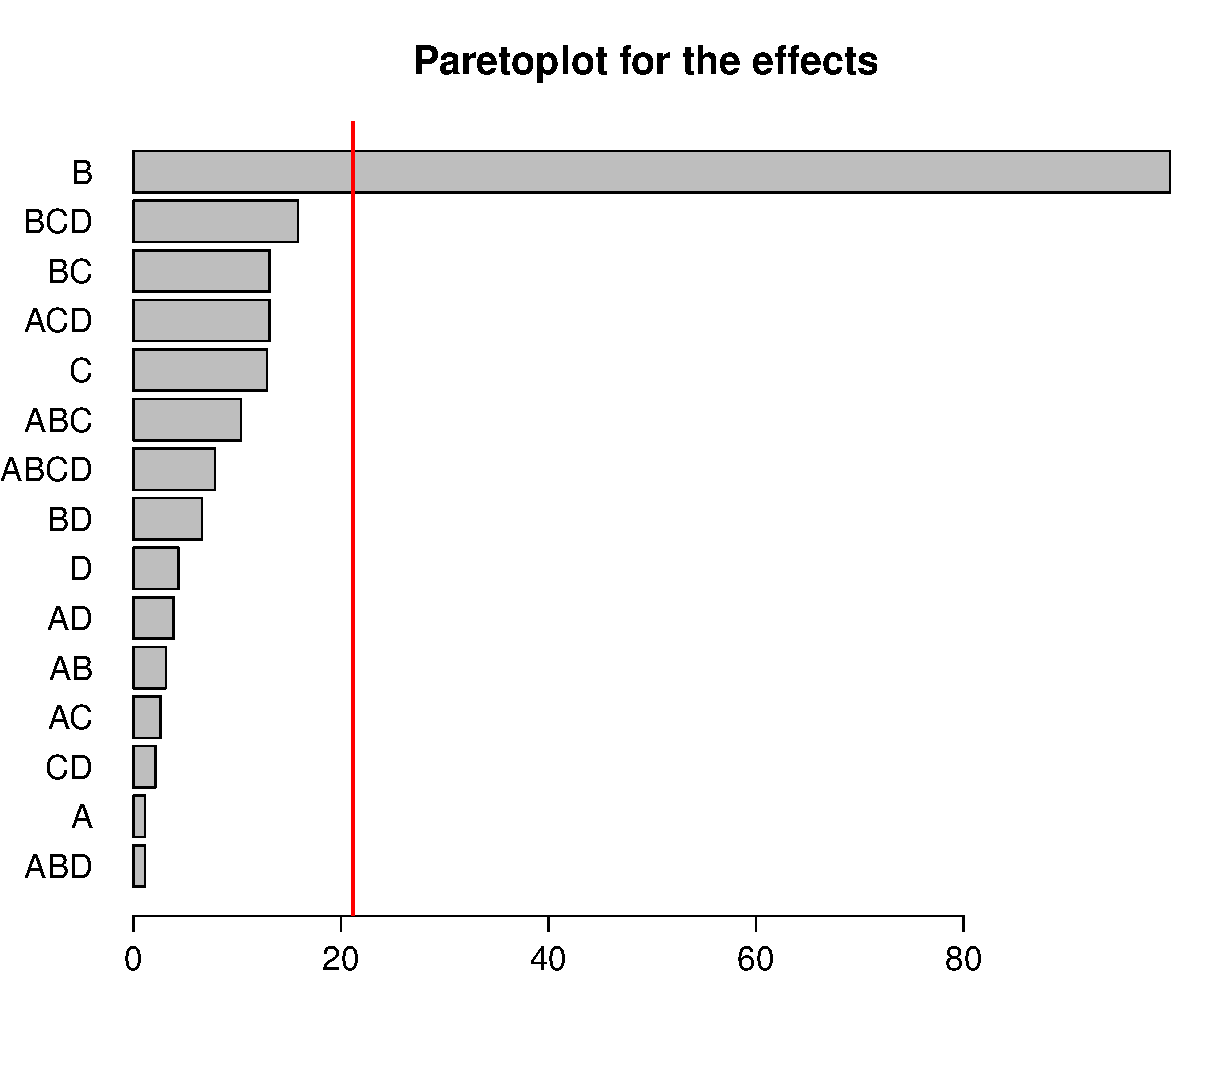
\includegraphics[width=0.6\textwidth]{PDF/paretoPlot.pdf}
    \caption{Awesome Image}
    \label{fig:awesome_image}
\end{figure}

\begin{figure}[p]
    \centering
    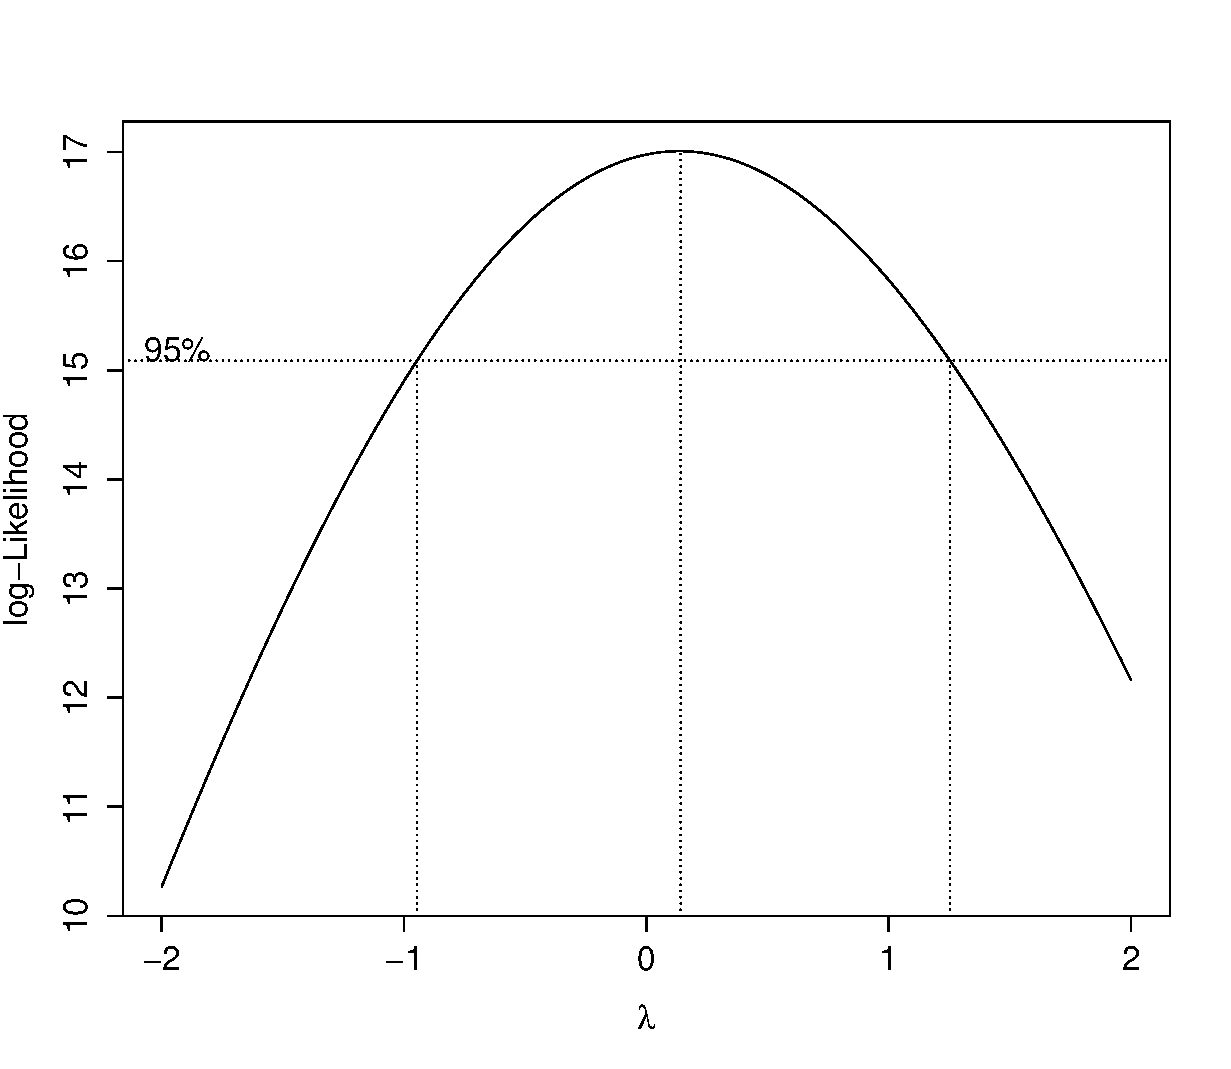
\includegraphics[width=0.6\textwidth]{PDF/boxCox.pdf}
    \caption{Awesome Image}
    \label{fig:awesome_image}
\end{figure}

\begin{figure}[p]
    \centering
    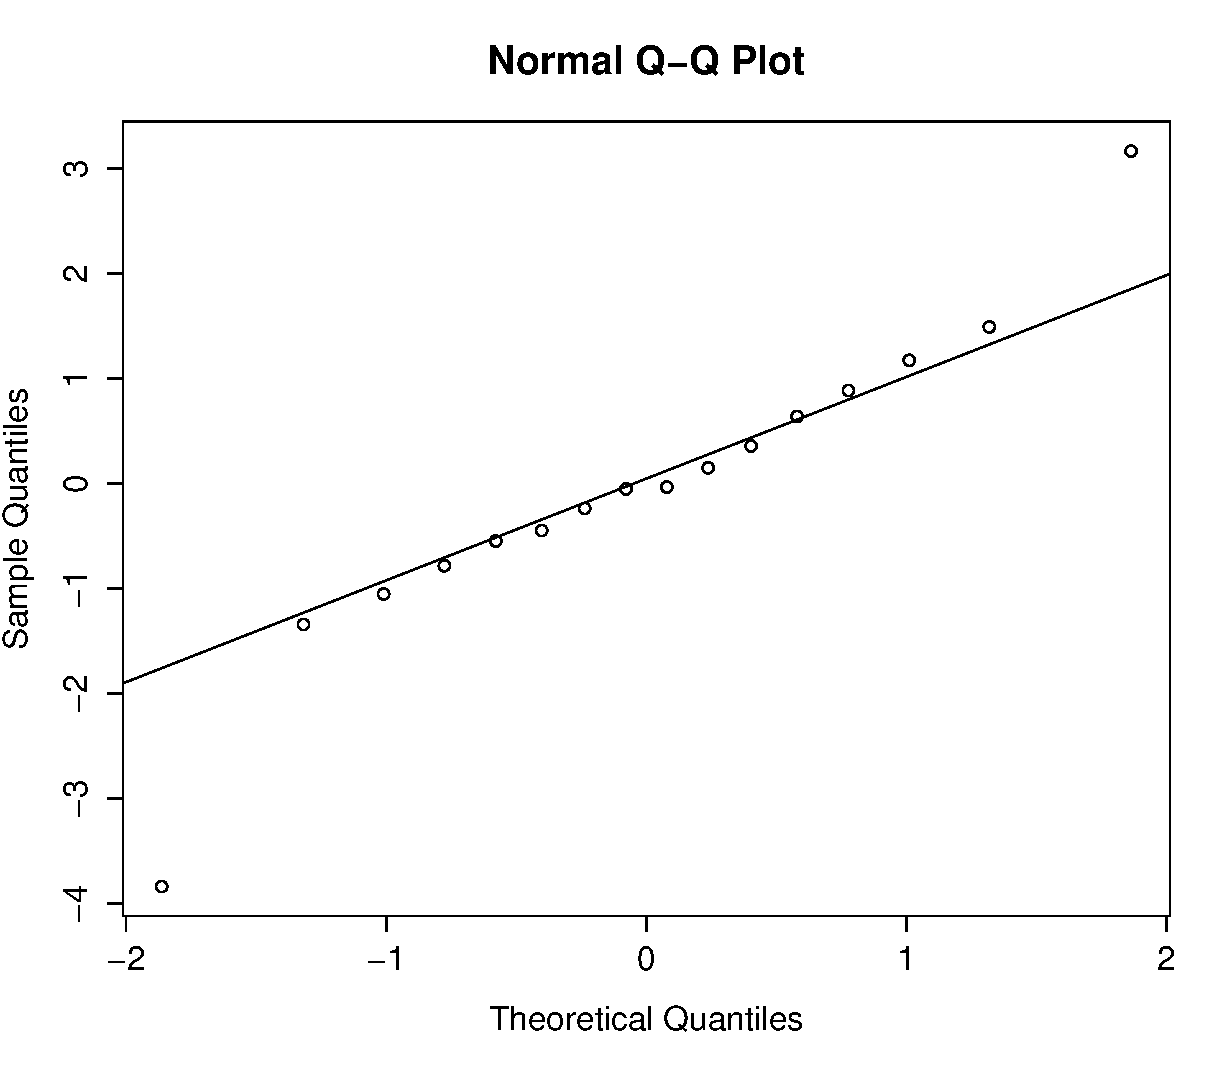
\includegraphics[width=0.6\textwidth]{PDF/qqPlot.pdf}
    \caption{Awesome Image}
    \label{fig:awesome_image}
\end{figure}

\begin{figure}[p]
    \centering
    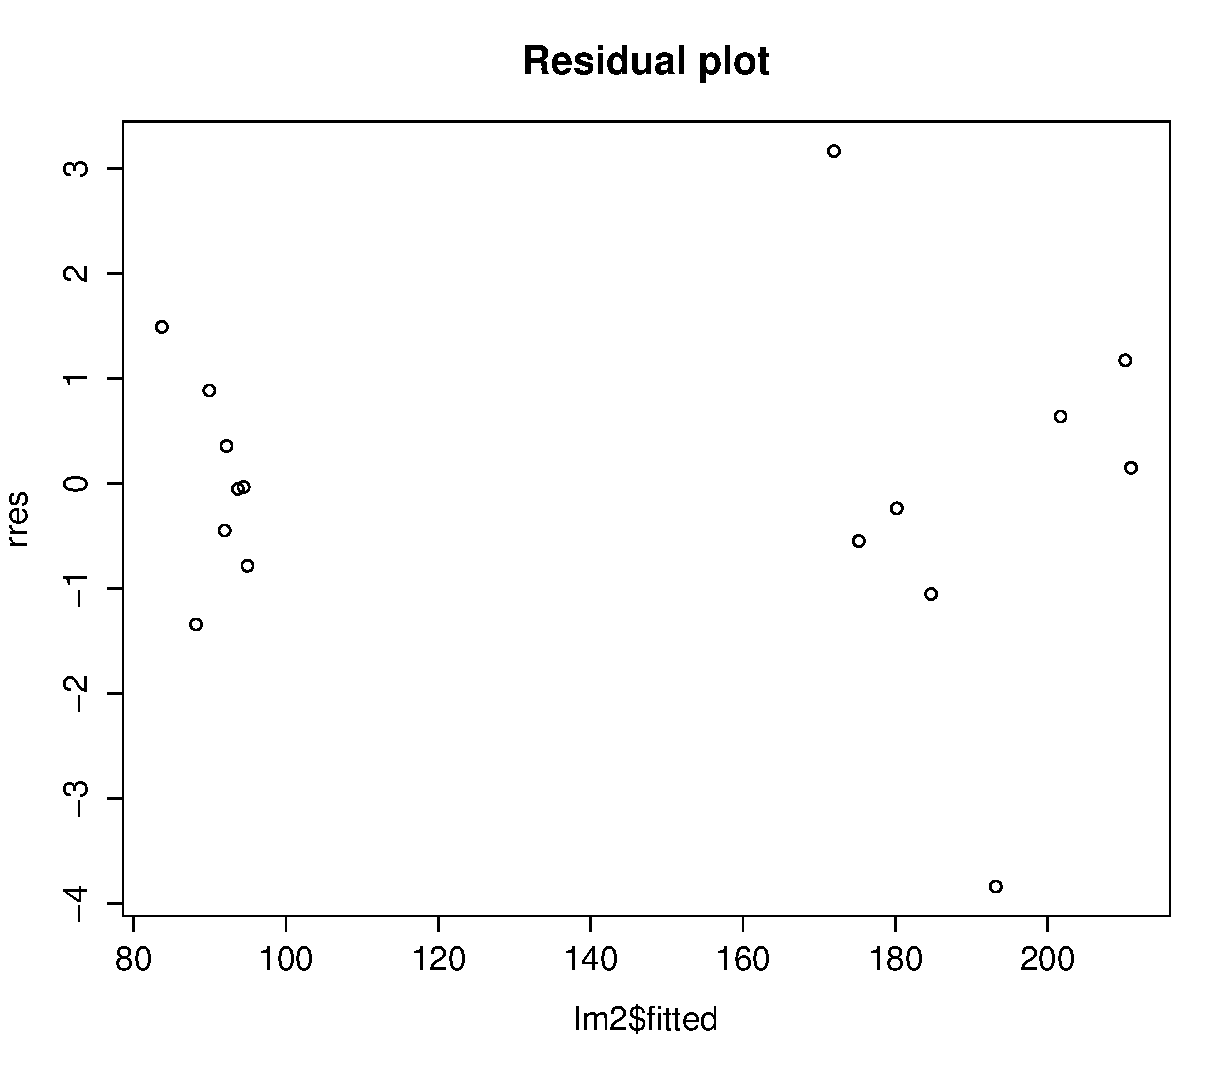
\includegraphics[width=0.6\textwidth]{PDF/residualPlot.pdf}
    \caption{Awesome Image}
    \label{fig:awesome_image}
\end{figure}

\begin{figure}[p]
    \centering
    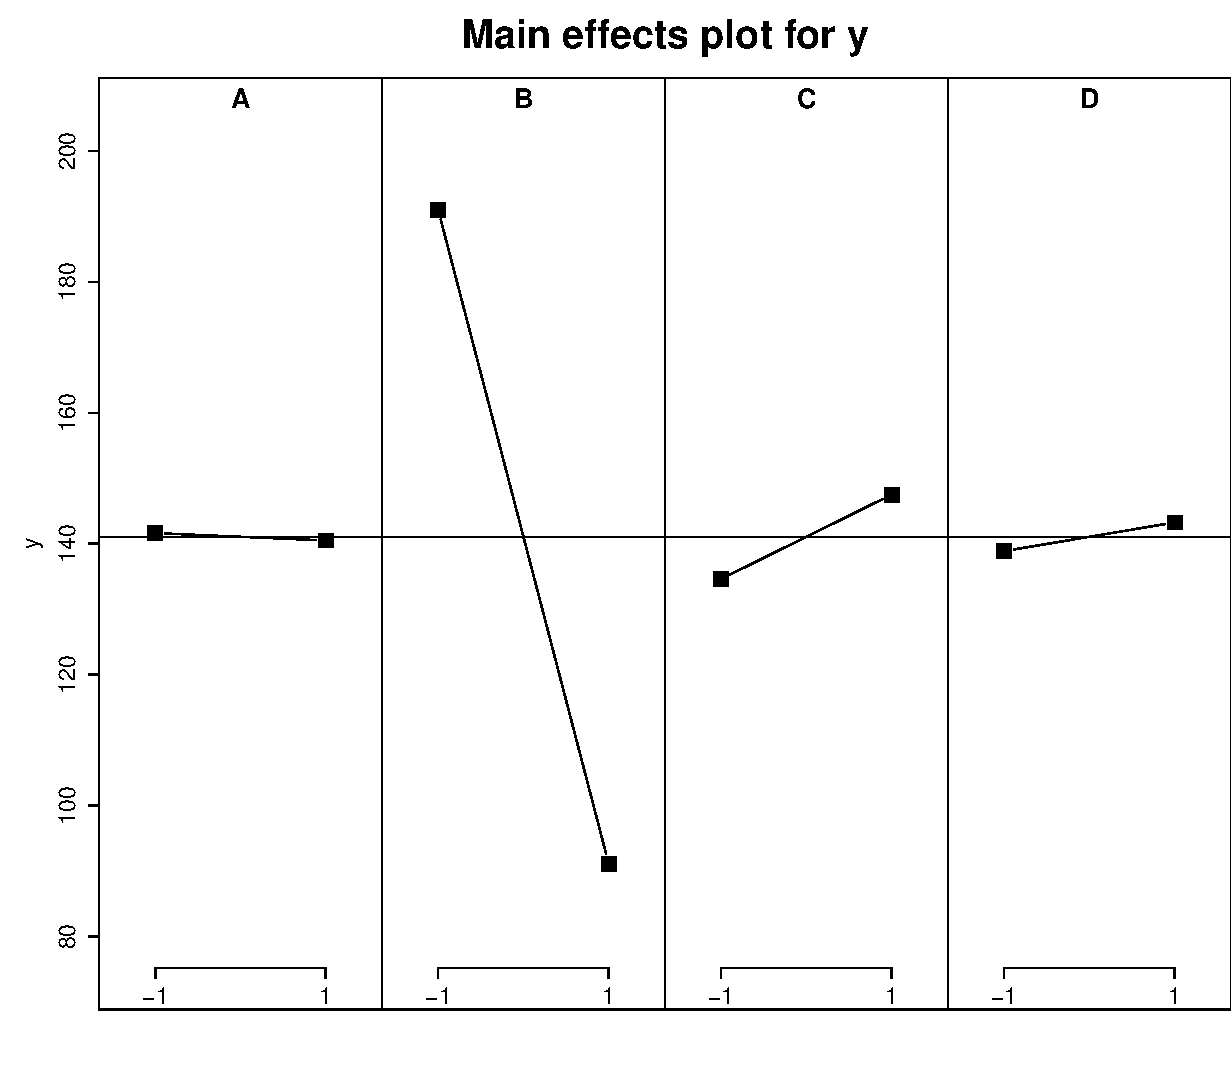
\includegraphics[width=0.6\textwidth]{PDF/mainEffects4factors.pdf}
    \caption{Awesome Image}
    \label{fig:awesome_image}
\end{figure}

\begin{figure}[p]
    \centering
    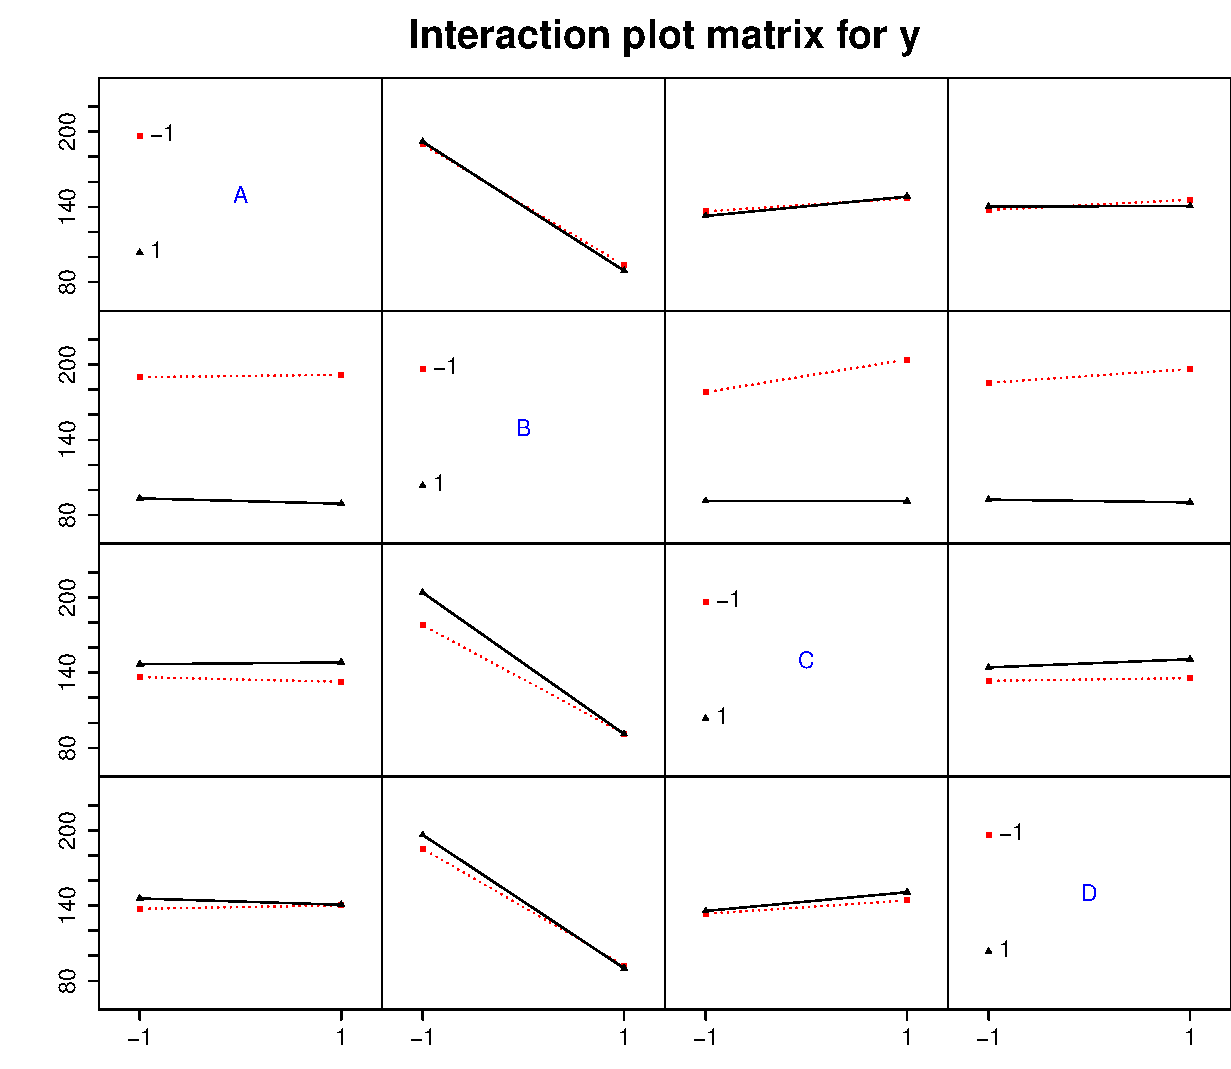
\includegraphics[width=0.6\textwidth]{PDF/interactionPlot4factors.pdf}
    \caption{Awesome Image}
    \label{fig:awesome_image}
\end{figure}
